\section{EiffelStudio}
EiffelStudio is a full-featured, commercial grade IDE for the Eiffel Programming Language (\cite[Quote from Origo website]{eiffel2006}). It has many tools to ease up designing systems with Eiffel and is focused on providing an "all-in-one" package for the user, so that no outside software is needed.

\subsection{The system}
EiffelStudio is build up with three main sections; libraries, framework, application (as seen in figure \ref{fig:eiffelstudio_structure}). This project is mainly focused in the UI subsection of application, more specifically, the tools part.
\begin{figure}[h]
\centerline{
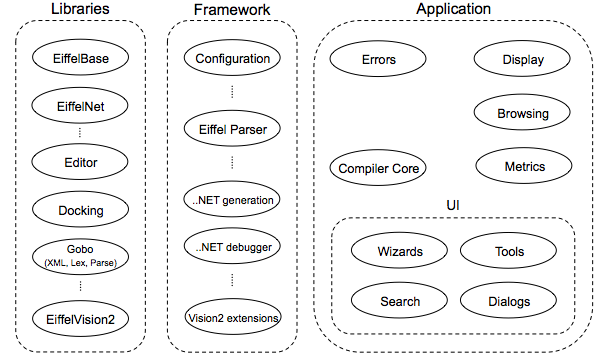
\includegraphics[scale=0.7]{images/eiffelstudio-structure-full.png}
}
\caption[Overview of the EiffelStudio structure]{Overview of the EiffelStudio structure (source: EiffelStudio presentation by Emmanuel Stapf).}
\label{fig:eiffelstudio_structure}
\end{figure}
\paragraph{}
The textual \textsc{bon} tool is implemented in a view (the reason for this will be explained in section \ref{why_a_view}). Switching between views is taken care of by a \textsc{eb$\textunderscore$development$\textunderscore$window}, through telling a \textsc{eb$\textunderscore$class$\textunderscore$text$\textunderscore$formatter} that it is now active. Such a \textsc{eb$\textunderscore$class$\textunderscore$text$\textunderscore$formatter} represents a view, but the \textsc{eb$\textunderscore$development$\textunderscore$window} does not know which \textsc{eb$\textunderscore$class$\textunderscore$text} \textsc{$\textunderscore$formatter} it is switching to as this is done polymorphic. It simply iterates through all its available formatters and waits for a \textit{selected}-flag to be set. When adding a new view one therefore has to add the new view to this collection of formatters and make sure the \textsc{ui} sets its \textit{selected}-flag appropriately. We the right \textsc{eb$\textunderscore$class$\textunderscore$text$\textunderscore$formatter} has been found the \textsc{format} feature will be invoked in order to start the formatting process for the chosen view.

\paragraph{}
This is how the \textsc{bon} tool is hooked into EiffelStudio as a view. The \textsc{bon} formatters, \textsc{textual$\textunderscore$ bon$\textunderscore$formal$\textunderscore$formatter} and \textsc{textual$\textunderscore$bon$\textunderscore$infor- mal$\textunderscore$formatter}, are added to the \textsc{eb$\textunderscore$development$\textunderscore$window}. A \textsc{eb$\textunderscore$sha- red$\textunderscore$format$\textunderscore$tables} then binds the formatter and a \textsc{class$\textunderscore$text$\textunderscore$formatter} together by instantiating the \textsc{class$\textunderscore$text$\textunderscore$formatter}, setting certain meta data on it and telling it to format with the formatter. This \textsc{class$\textunderscore$text$\textunderscore$formatter} executes the formatter, which hands over an abstract eiffel syntax representation of the class in scope to a \textsc{textual$\textunderscore$bon$\textunderscore$formal$\textunderscore$output$\textunderscore$strategy} which starts the actual extraction of \textsc{bon}. An overview of  an example of this structure for formal textual \textsc{bon} can be seen in figure \ref{fig:extractor_structure}.
\begin{figure}[h]
\centerline{
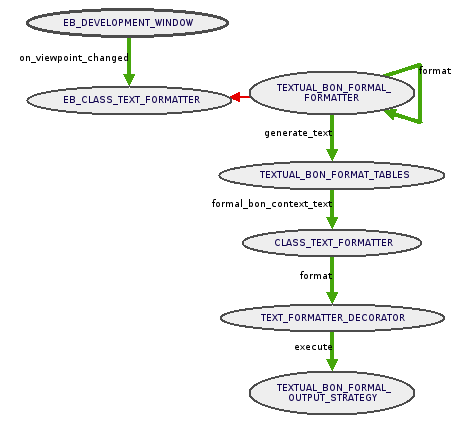
\includegraphics[scale=0.7]{images/BON-extractor-structure-large.png}
}
\caption{Structure of the BON extractor's interaction with EiffelStudio for formal BON.}
\label{fig:extractor_structure}
\end{figure}

\subsubsection{Why in a view?}
\label{why_a_view}
EiffelStudio has multiple ways of showing the same code. This is taken care of by the view feature. While viewing a piece of Eiffel code, you can switch to i.e. the interface view, where you can see the signature, comments and contracts of both own, but also inherited features. This gives the user the ability to see a class' overall structure, through showing information not normally available, and hiding information that is not relevant to the view. In the case of the interface view, the body of features is hidden to ensure a proper overview and to remove clutter from viewing too many features at once.
\paragraph{}
A \textsc{bon} tool's function is similar to this in many ways. It allows the user to see the code from a textual \textsc{bon} perspective, with the idea of charts (informal) and components (formal) to help giving an overview of the structure of the code. The exact functionality of the \textsc{bon} tool will be discussed in later sections. Due to this similarity between the currently implemented views and the \textsc{bon} tool, having this new tool as an added view makes it feel apart of EiffelStudio, and not some external tool.

\subsection{BON syntax highlighting}